\begin{frame}
\frametitle{Transatomic Power (TAP) concept high-fidelity Serpent model}
	  \begin{textblock*}{12.25cm}(0.25cm,1.8cm) % {block width} (coords)
\begin{figure}[htp!] % replace 't' with 'b' to 
	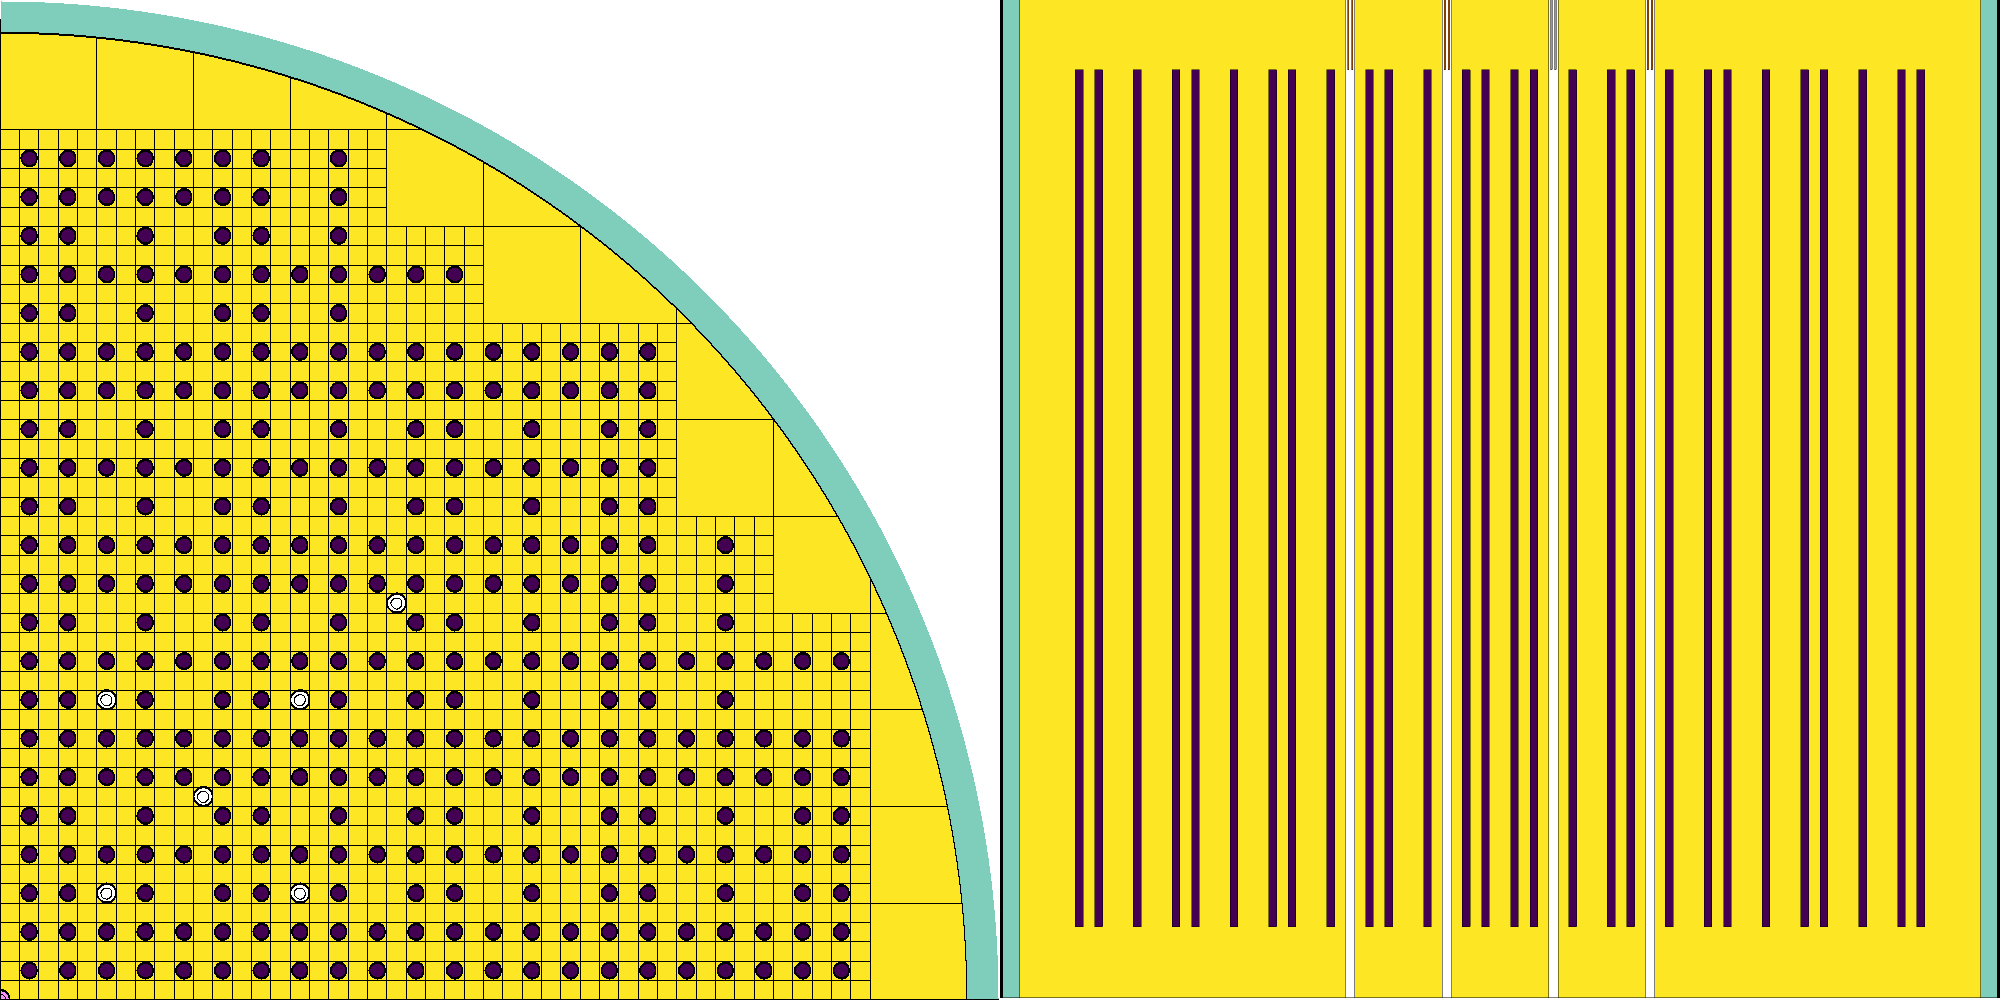
\includegraphics[width=\textwidth]{./images/tap_model.png}
	\caption{An $XY$ (left) and $XZ$ (right) section of the TAP model. 
	The violet color represents zirconium hydride, and the yellow represents 
	fuel salt (reproduced from Rykhlevskii \& Huff, Milestone 2.1 Report, 
	2019).}
\end{figure}
	  \end{textblock*}
\end{frame}


\begin{frame}
\frametitle{Depletion simulation results for TAP with various feeds}       
\begin{textblock*}{12.6cm}(0.1cm,2.2cm) % {block width} (coords)
	\begin{figure}[htp!] % replace 't' with 'b' to 
		\begin{minipage}[b]{0.48\textwidth}
			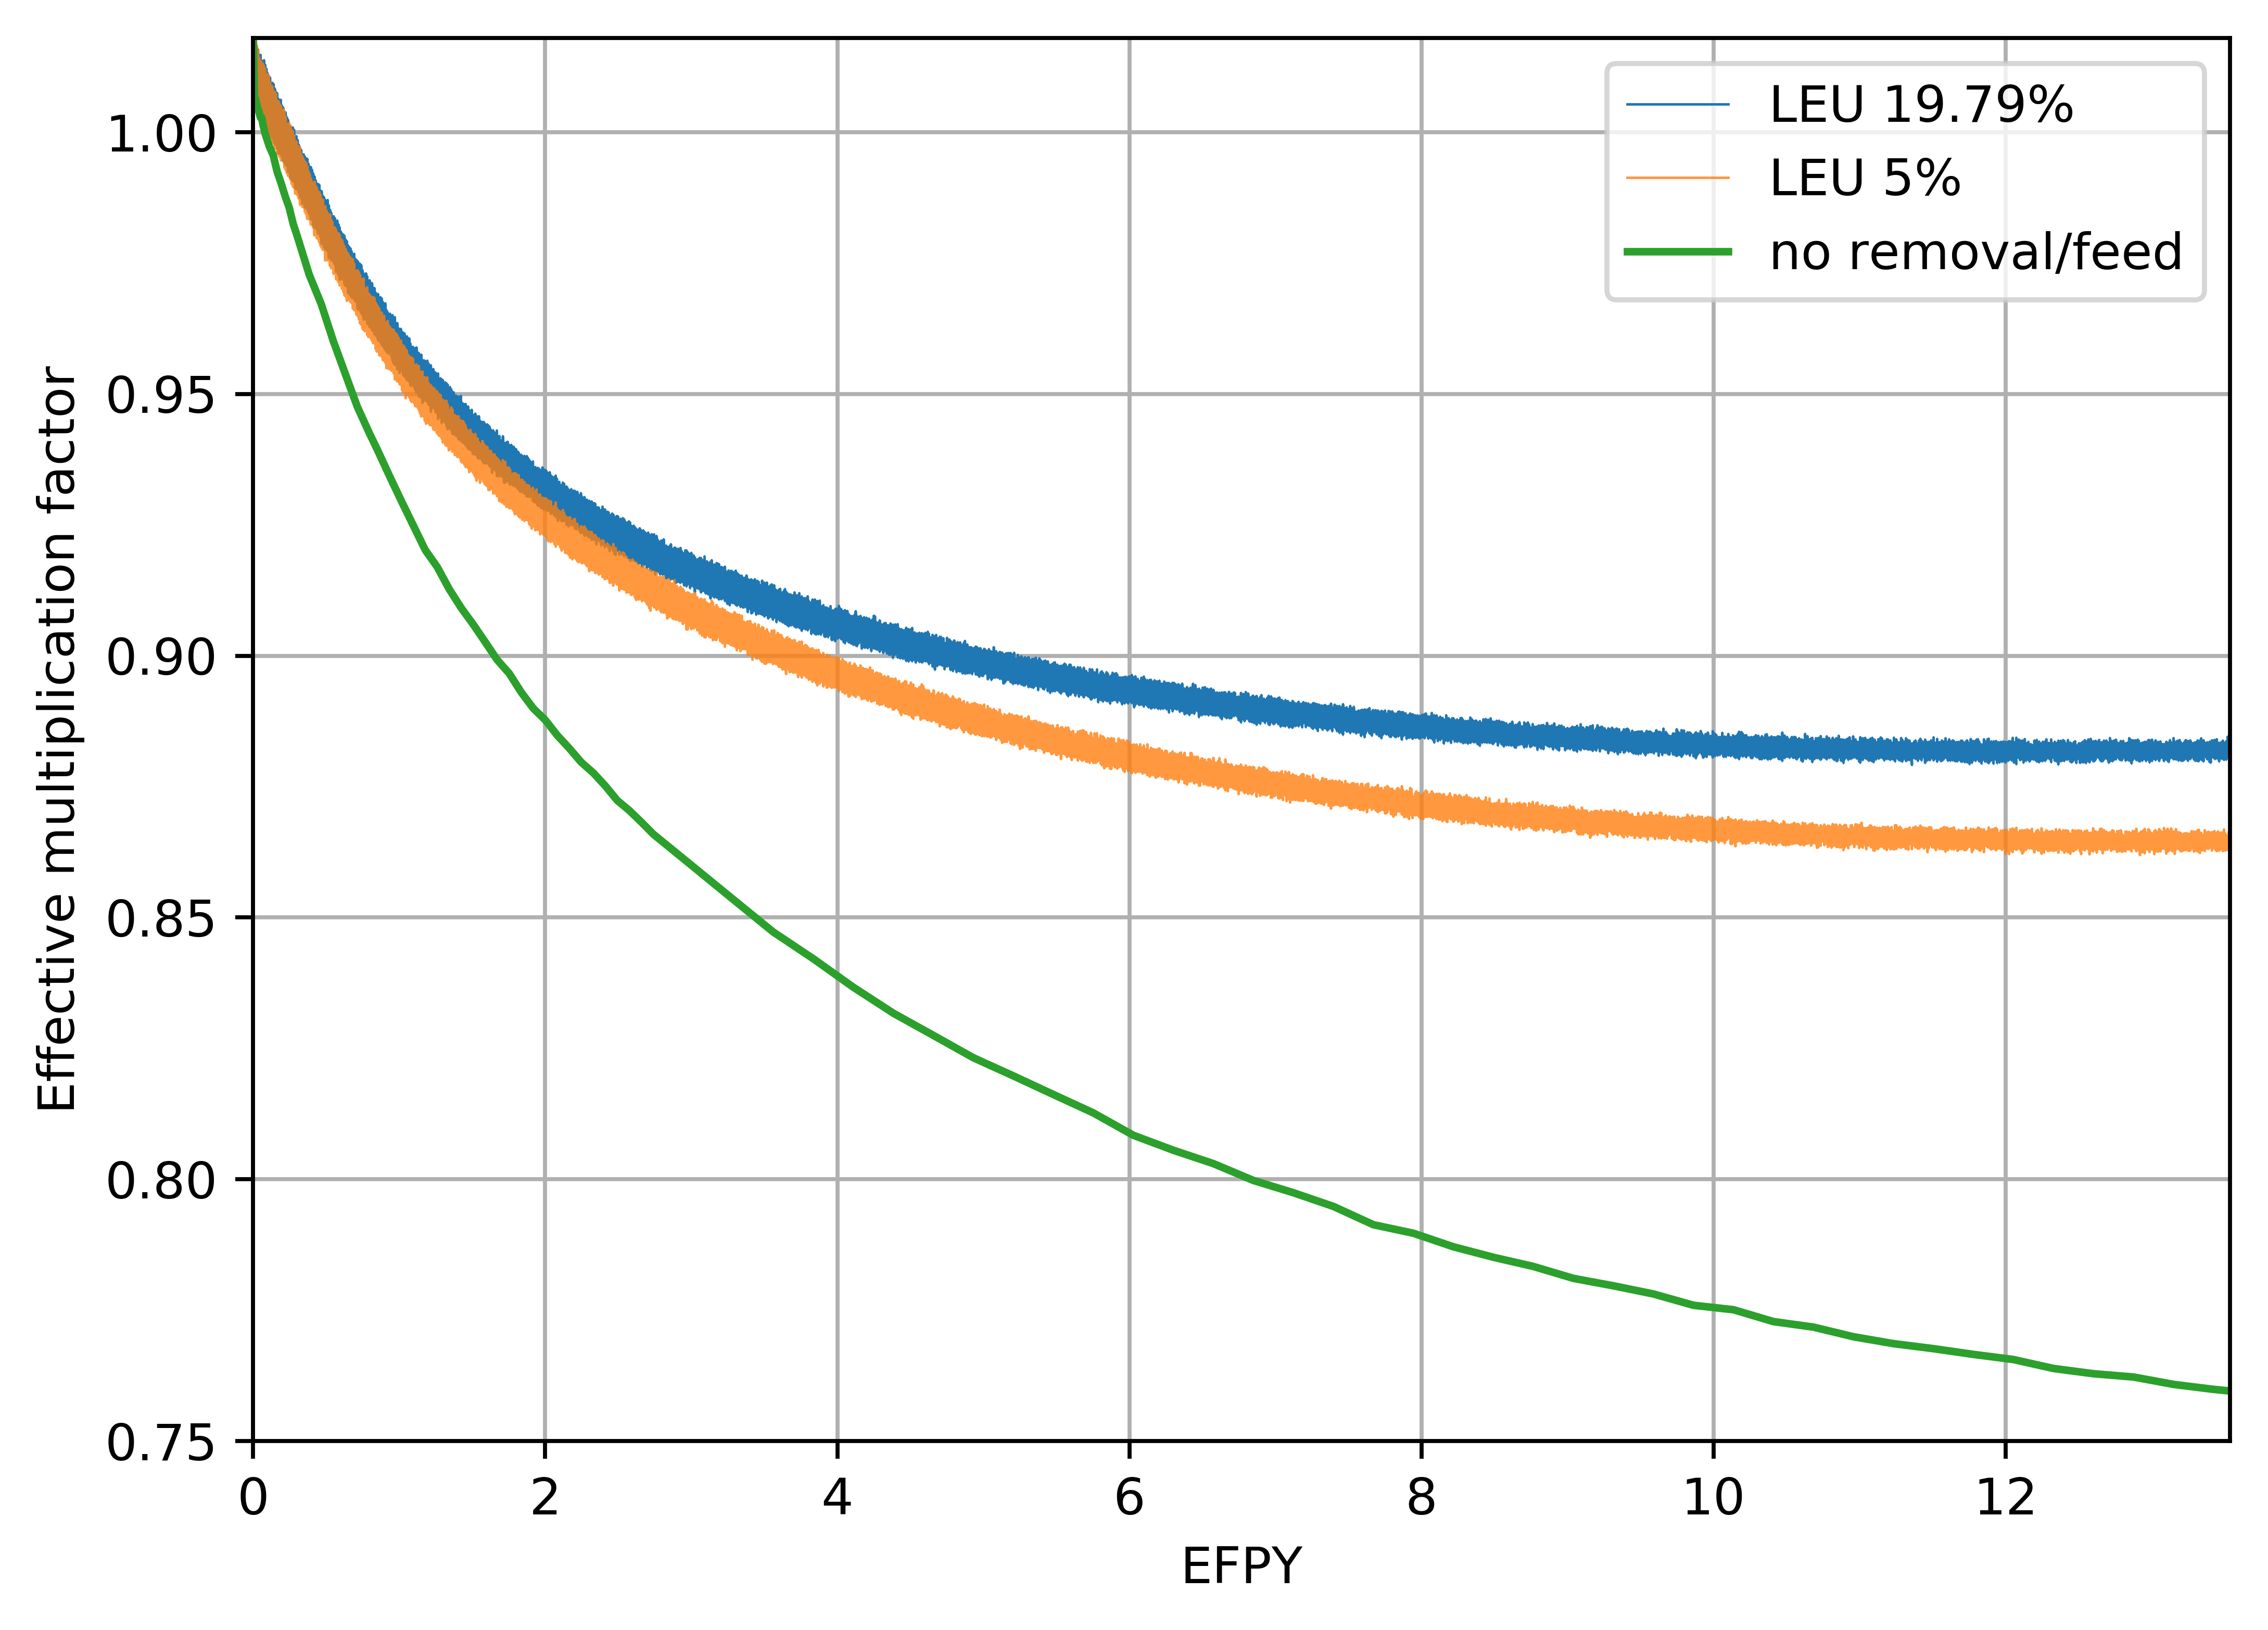
\includegraphics[width=\linewidth]{./images/keff_3.png}
		\end{minipage}
			\hspace{-2mm}
		\begin{minipage}[b]{0.48\textwidth}
			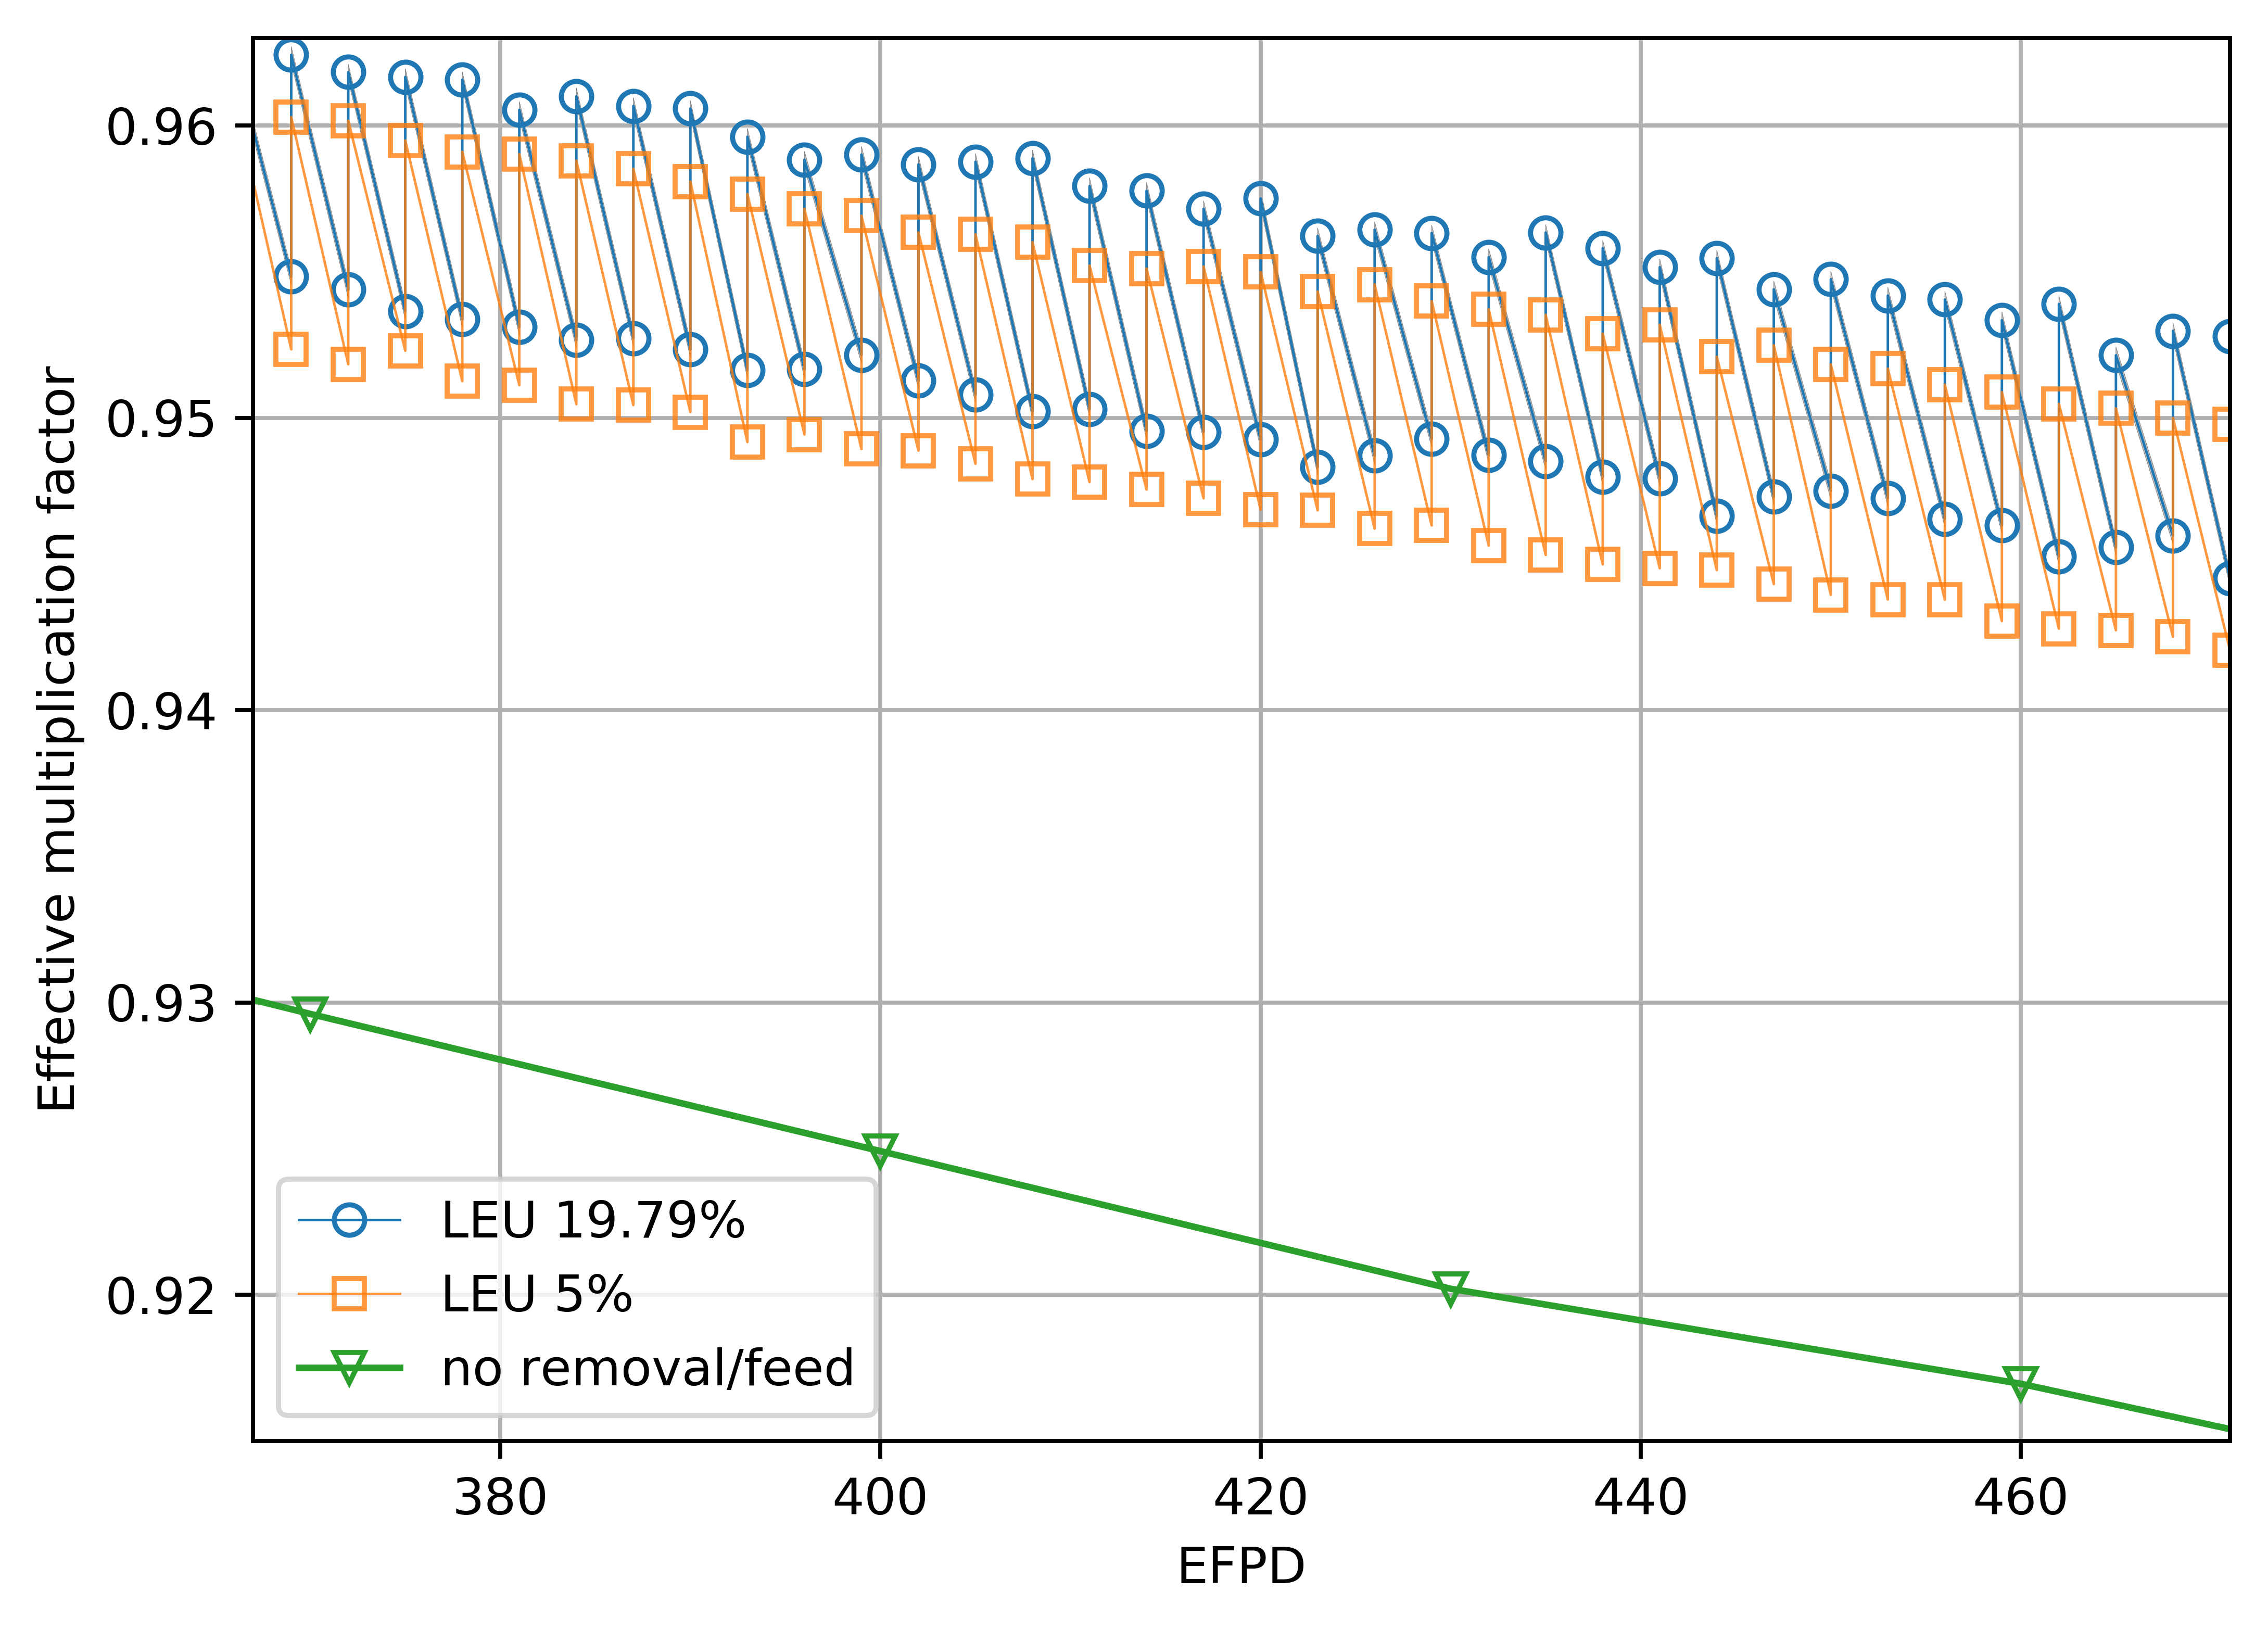
\includegraphics[width=\linewidth]{./images/keff_zoomed_2.png}
		\end{minipage}
		\caption{Effective multiplication factor dynamics for full-core
		TAP model for different fueling scenarios over a 13-year reactor 
		operation (left) and for the time interval from 367 to 471 days after 
		startup (right). Confidence interval $\pm\sigma=28pcm$ is shaded.}
	\end{figure}
\end{textblock*}
\end{frame}


\begin{frame}
\frametitle{Fuel salt composition evolution during the TAP operation}
\begin{textblock*}{12.25cm}(0.25cm,2cm) % {block width} (coords)
	\begin{figure}[htp!] % replace 't' with 'b' to 
		\centering
				\vspace{-3mm}
		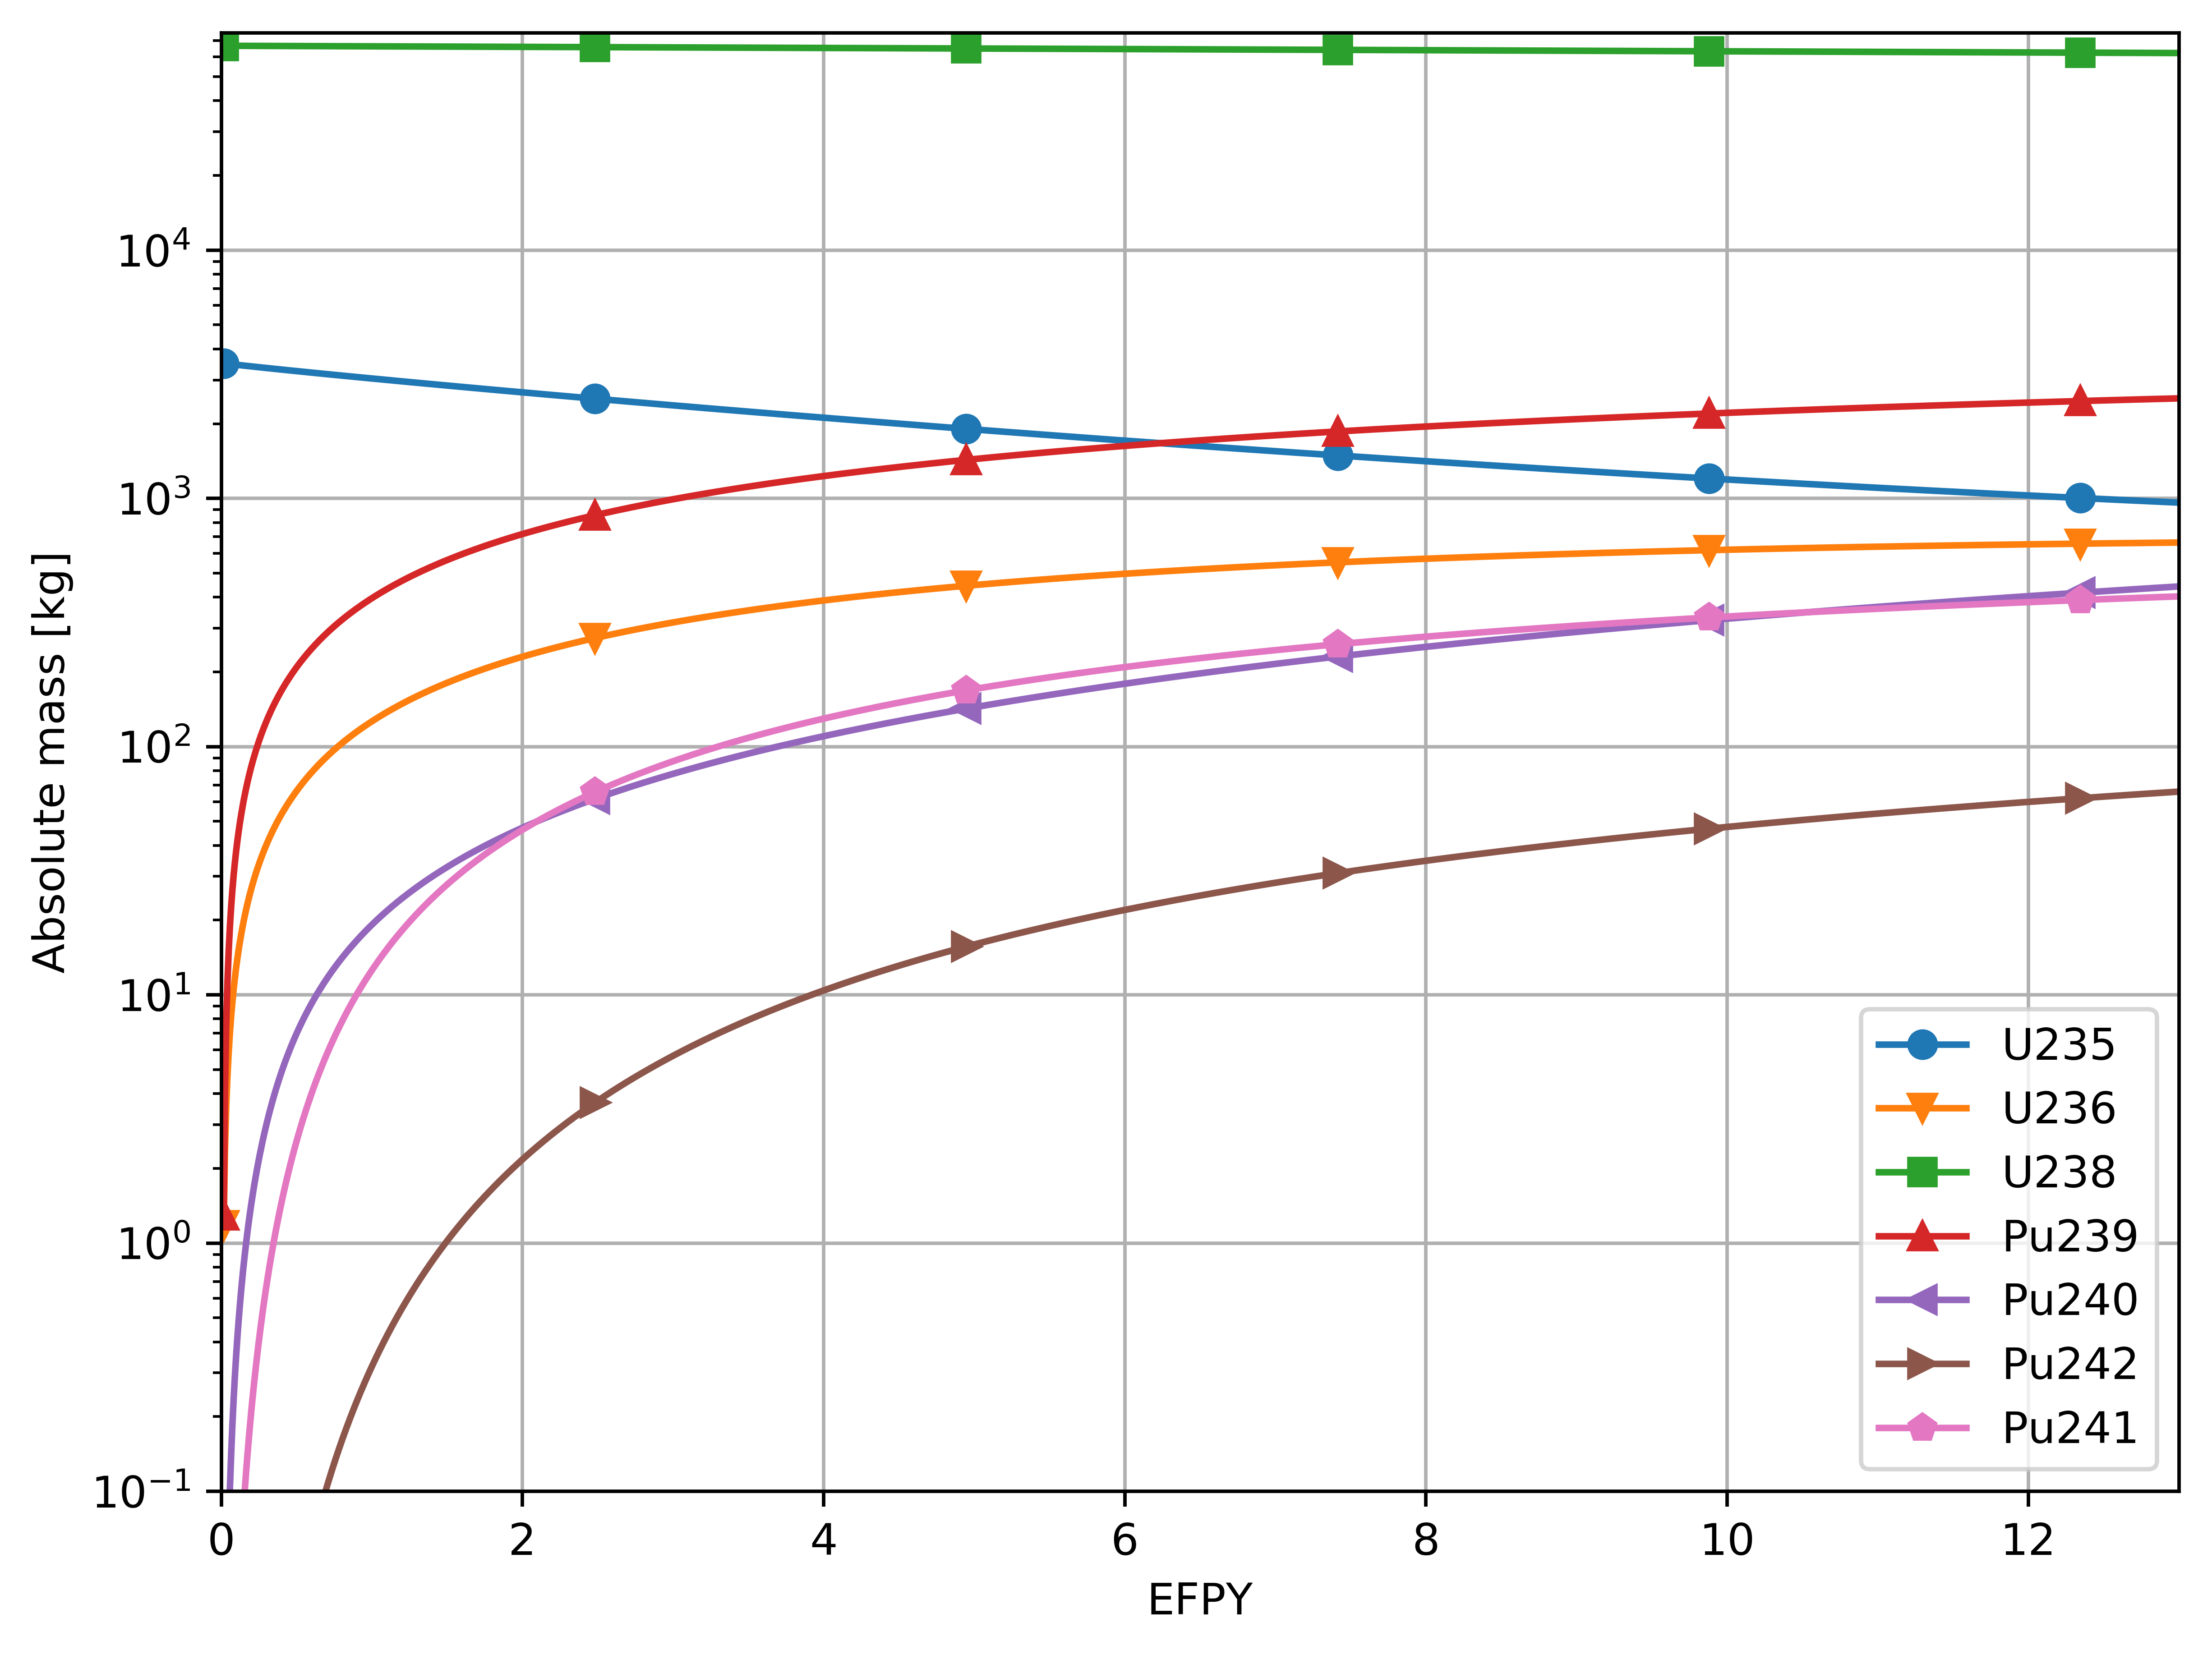
\includegraphics[width=0.72\textwidth]{../images/u_pu_mass.png}
		\caption{Mass of major nuclides during 13 years of reactor operation 
		with 19.79\% low-enriched uranium feed.}
	\end{figure}
\end{textblock*}
\end{frame}